
\section{Johdanto}

Ohjelmistoalan kilpailutilanteen kiristyessä yritykset etsivät jatkuvasti tapoja
tehostaa toimintaansa. Ketterien menetelmien on todettu parantavan tehokkuutta
sekä laatua \citeppri{Livermore2008}, mikä nostaa ne houkuttelevaksi vaihtoehdoksi
tehostamista tavoitteleville yrityksille. Ketterien menetelmien käyttöönotto on
kuitenkin haastavaa suurissa yrityksissä \citeppri{Dyba2009}. Alun perin pieniin
projekteihin ja tiimeihin\footnote{Tässä työssä käytetään ohjelmistoalalla
vakiintunutta lainasanaa tiimi (engl. team) viitaten projektin työryhmään.}
suunnitellut mallit ovat osoittautuneet vaikeiksi soveltaa suuremmassa
mittakaavassa \citeppri{Boehm2005}.

Suuret yritykset toimivat usein perinteisten ohjelmistotuotannon mallien
mukaisesti. Nämä mallit pyrkivät optimoimaan toimintaa tarkalla suunnittelulla
ja prosessien määrittelyllä. Tämänlainen lähtökohta soveltuu kuitenkin huonosti
ohjelmistokehitykseen, sillä kehitysprojekteissa syntyy lähes poikkeuksetta
tilanteita, joita on mahdotonta tai liian työlästä ennustaa \citeppri{Schwaber2002}.
Suurimpia ongelmia suunnitelmavetoisissa menetelmissä on vaatimusten muuttamisen
korkea hinta sekä myöhäinen palaute tuotteen laadusta \citeppri{Petersen2010}.
Pitkät julkaisuvälit, muutoksiin vastaamisen kalleus sekä etäisyys asiakkaista
heikentävät yritysten kilpailukykyä. Apua näihin ongelmiin toivotaan löytyvän
ketterien kehitysmallien soveltamisesta.

Tämän työn tavoite on esittää nykyinen tutkimuksen tila ketterien
ohjelmistokehitysmenetelmien käyttöönotosta suurissa organisaatioissa,
tarkastellen erityisesti siihen liittyvää organisaatiomuutosta. Ketterien
menetelmien käyttöönotosta on olemassa tutkimuksia, mutta ne keskittyvät
enimmäkseen pieniin organisaatioihin tai yksittäisiin tiimeihin. Suuret
organisaatiot mukautuvat uusiin menetelmiin hitaammin, mikä voidaan olettaa
syyksi siihen, että laajaa tutkimusta suuren mittakaavan ketterästä muutoksesta
ei ole aikaisemmin tehty.

Tämä työ on toteutettu mukaillen järjestelmällisen kirjallisuustutkimuksen
muotoa, kartoittaen olemassa olevat tapaustutkimukset ja kokemusraportit.
Tutkimuskysymys, johon tässä työssä vastataan on: Mitkä tekijät vaikuttavat
ketterän kehitysmallin organisaatiomuutoksen läpiviemiseen suuressa
organisaatiossa? Työn tulos osoittaa, että ketterien kehitysmenetelmien
käyttöönotosta suurissa organisaatioissa on olemassa riittävästi ensisijaisia
tutkimuksia kirjallisuustutkimukseen.

Luvussa \ref{sec:tausta} esitellään aikaisempia tutkimuksia liittyen tämän työn
aihealueeseen, sekä todetaan, että työ vastaa olemassa olevaan aukkoon
tutkimuksessa. Luvussa \ref{sec:menetelma} on esitelty järjestelmällisen
kirjallisuustutkimuksen menetelmä, sekä tapa jolla sitä on sovellettu tämän
kandidaatintyön kokeellisena osiona. Luvussa \ref{sec:tulokset} käsitellään
kirjallisuustutkimuksen tulokset. Lopuksi esitellään tuloksista tehdyt
johtopäätökset sekä työn yhteenveto.


% --------------------------------------------------------------------
\clearpage
\section{Työn taustat}
\label{sec:tausta}

Tämän työn tavoitteena on kuvata ketterien kehitysmenetelmien käyttöönoton
perusteita, haasteita ja menestyksen tekijöitä suurissa organisaatioissa.
Taustatietona tässä luvussa esitellään havaintoja edellisistä tutkimuksista,
jotka liittyvät ketterien menetelmien käyttöönoton haasteisiin, sekä suuren
mittakaavan ketterään kehitykseen. Myös ketterien menetelmien menestyksekkään
käyttöönoton tekijöitä esitellään. Luvun lopuksi perustellaan tämän työn
merkitys suhteessa olemassa olevaan tutkimukseen.

\subsection{Ketterä ohjelmistokehitys}

Ketterä ohjelmistokehitys on joukko menetelmiä, jotka on kehitetty vaihtoehdoksi
niin kutsutulle perinteiselle suunnitelmavetoiselle kehitykselle. Ketterien
menetelmien näkökulmasta perinteiset mallit pyrkivät vähentämään muutoksia
tuotteen kehityksessä ja tulkitsevat muutoksia virheinä. Tuotteen
mukautumiskyky kehityskaaren aikana ja kyky vastata arvaamattoman maailman
haasteisiin ovat nykyään kuitenkin kriittisiä tekijöitä. Muutoksen omaksuminen
kehityksessä, korkean laadun tavoitteleminen ensi askelista alkaen sekä
ihmiskeskeisyys ovat ketterien menetelmien keskeisiä teemoja.
\citeppri{Highsmith2001}

Ketterää kehitystä on sekä kritisoitu että puollettu, ja tutkimukset ovat
osoittaneet muutoksen omaksumisen sekä menestyksen että epäonnistumisen
tekijöinä \citeppri{Boehm2002}. On osoitettu, että ketterät menetelmät ovat
parantaneet sekä kehittäjien että asiakkaiden tyytyväisyyttä, mutta toisaalta on
olemassa todisteita siitä, että ketterät menetelmät eivät välttämättä sovellu
suuriin hankkeisiin \citeppri{Dyba2009}. \citepri{Boehm2002} ehdottaakin, että
organisaatioiden tulisi etsiä itselleen sopiva tasapaino suunnitelmavetoisten ja
ketterien menetelmien välillä.

Nykyään yleisiä ketterän kehityksen menetelmiä ovat Scrum ja Extreme Programming
(XP) \citeppri{Dyba2008}. Scrum on projektinhallintamenetelmä, joka painottaa
tiimikeskeistä toimintaa, ajallista rytmittämistä (time-boxing), jatkuvaa
edistymisen seurantaa sekä asiakaskeskeisyyttä \citeppri{Schwaber2002}.
XP-menetelmä perustuu kokoelmaan käytäntöjä, joista keskeisimmät ovat jatkuva
palaute kehityksestä, testausvetoinen kehitys, asiakkaan jatkuva mukanaolo,
pariohjelmointi ja jatkuva yhdentäminen (engl. Continuous Integration
CI) \citeppri{Beck1999}.

Ketterän kehitysmallin rinnalla on olemassa myös kevyt kehitysmalli (engl. lean
development). Kevyt kehitys tähtää, samoin kuin esimerkiksi XP- ja
Scrum-menetelmät, panostamaan niihin toimintoihin, jotka tuottavat arvoa
asiakkaalle. Kevyen kehityksen keskeisiä periaatteita ovat kokonaisuuden
optimointi, hukkatuotannon (engl. waste) poistaminen, laadun rakentaminen
tuotteen sisään sekä jatkuva tiedon jakaminen ja oppiminen.
\citeppri{Poppendieck2012}.

\subsection{Ketterien menetelmien käyttöönoton haasteita}

Ketterien menetelmien käyttöönotto ei perustu yksittäisiin uusiin
toimintatapoihin tai työkaluihin, vaan kokonaisvaltaiseen toiminta- ja
ajattelutavan muutokseen. Tämänlainen muutos vaatii koko organisaatiokulttuurin
muuttumista \citeppri{Misra2009}, mikä on haastavampaa kuin pelkästään uusien
työkalujen käytön opetteleminen. Muutosta saattaa vaikeuttaa
suunnitelmavetoiseen toimintamalliin juurtuneet ajattelutavat ja asenteet
\citeppri{Mahanti2006,Nerur2005}. Ketterässä kehityksessä organisaatiokulttuurin
on oltava tiimi- ja asiakaskeskeinen, tiimeillä pitää olla valinnanvapaus
työkalujen ja menetelmien käytössä ja tiedon välittyminen pitää mahdollistaa
myös muissa muodoissa kuin kirjoitettuna dokumentaationa \citeppri{Misra2009}.

Kehittäjät ovat keskeisessä roolissa ketterissä malleissa. Organisaatiossa
joissa on vahva tausta suunnitelmavetoisesta kehityksestä saattaa kehittäjien
osaaminen olla kapea-alaista, mikä muodostuu ongelmaksi ketterien menetelmien
vaatiessa enemmän yleisiä taitoja \citeppri{Nerur2005}. Keskeinen ominaisuus,
jota kehittäjien tulisi osoittaa ketterissä malleissa, on itseohjautuvuus
\citeppri{Misra2009}. Ketterien menetelmien yhteydessä on suositeltu keskivertoa
parempien kehittäjien käyttämistä \citeppri{Boehm2002}. Pelkästään
huippukehittäjien käyttäminen ei ole välttämätöntä, mutta heikoimpien
suoriutujien mukanaolo on haitallista ketterässä kehityksessä
\citeppri{Nerur2005,Boehm2005}. Muutoksen myötä kehittäjien on omaksuttava uusia
työtapoja, mikä saattaa aiheuttaa muutosvastarintaa. Eräitä syitä
muutosvastarintaan voivat olla pelko omien taitojen riittämättömyydestä uudessa
ympäristössä tai kateuden tunne työtovereiden uusista tehtävistä
\citeppri{Boehm2005}.

Tiimien prosessien lisäksi myös liiketoiminnan prosesseja joudutaan sopeuttamaan
ketteriin menetelmiin. Tuotannon ja suunnittelun tulisi etääntyä
elinkaariajattelusta ja painottaa iteratiivista ja toiminnallisuuksiin
keskittyvää mallia \citeppri{Nerur2005}. Ongelmana on, että perinteisissä
malleissa on annettu pitkän aikavälin suunnitelmia ja tehty sitoumuksia, mutta
ketterät menetelmät perustuvat nopeiden muutosten mahdollistamiseen. Tämän takia
organisaation johdon on hyväksyttävä muutosten tekeminen lyhyemmällä
aikajänteellä \citeppri{Misra2009}. Perinteisesti liiketoimintaa on ohjattu
pitkän tähtäimen suunnittelulla, mutta ketterät menetelmät painottavat, että
merkityksellistä suunnittelua voi tehdä vain lähitulevaisuuteen
\citeppri{Boehm2005}. Johdon on myös hyväksyttävä, että kehitystyötä ei kannata
pyrkiä hallitsemaan yksityiskohtaisella tasolla, vaan on sallittava esimerkiksi
kevyemmät raportointikäytännöt \citeppri{Cohn2003}.

Ketterät menetelmät vaativat asiakkaan vahvempaa läsnäoloa, mutta kaikki
asiakkaat eivät halua tai voi osallistua kehitykseen \citeppri{Nerur2005}.
Muodollisten dokumenttien puuttuessa asiakkailta vaaditaan luottamusta
kehitystiimiin, sekä joustavuutta neuvoteltaessa mahdollisista muutoksista
\citeppri{Misra2009}. Myös sopimuskäytäntöjä pitää muuttaa perustumaan toimivan
ohjelmiston toimittamiseen sen sijaan, että keskitytään muodollisiin
katselmointeihin tai dokumentaatioon \citeppri{Boehm2005}.

Suurissa organisaatioissa ketterien menetelmien käyttöönotto on haastavampaa
kuin pienissä \citeppri{Livermore2008,Dyba2008}. Tärkeä tekijä suurissa
organisaatioissa on se, että projektit ovat harvoin riippumattomia toisista.
Riippuvuudet kasvattavat tiimin tarvetta kommunikoida ulospäin. Suuri mittakaava
saattaa pakottaa ketteryyden vähentämistä esimerkiksi muodollista
dokumentaatiota lisäämällä \citeppri{Lindvall2004}. Ketterät menetelmät
saattavat myös joutua törmäyskurssille organisaation muiden toimintojen kanssa.
Muun muassa henkilöstöhallinnon käytännöt saattavat estää työntekijöitä
ottamasta uusia ja laajempia rooleja, mitä ketterä kehitys vaatii
\citeppri{Boehm2005}. Muutoksenhallintalautakunta (engl. change control board,
CCB) saattaa hankaloittaa koodin uudelleenjärjestämisen (engl. refactoring) ja
jatkuvan yhdentämisen käyttöä \citeppri{Lindvall2004}. Organisaation
kehitystyöhön liittymättömiä ryhmiä pitää informoida muutoksesta ketterään
kehitykseen, ja ketterää mallia pitää sovittaa toimimaan yhteen niiden kanssa
\citeppri{Lindvall2004,Cohn2003,Boehm2005}. Liittyminen ympäröivään
organisaatioon saattaa johtaa siihen, että on tuettava lopputuotteen kannalta
vähemmän arvoa lisääviä käytäntöjä, kuten dokumentaatiota ja jäykempää
suunnittelua \citeppri{Mahanti2006}.

\subsection{Menestyksekkään käyttöönoton tekijöitä}

Ketterien menetelmien käyttöönotossa kannattaa seurata organisaatiomuutoksiin
yleisesti liittyviä hyviä käytäntöjä. Näitä ovat johdon myötämielisyys
muutokselle, pilottiprojektien käyttö sekä henkilöstön kouluttaminen.

Johdon myötämielisyydellä ja osallistumisella on merkittävä vaikutus
onnistumiseen, kun muutetaan ohjelmistokehityksen toimintatapoja
\citeppri{Livermore2008}. Ketterän kehityksen lupaama tehokkuuden kasvu
houkuttelee johtoa tukemaan ketterien menetelmien käyttöönottoa, erityisesti jos
aikaisempien projektien on havaittu ylittäneen budjetteja tai aikarajoja
\citeppri{Cohn2003}. Käyttöönoton riskejä on järkevää vähentää kokeilemalla
ketteriä menetelmiä lyhyillä pilottiprojekteilla \citeppri{Lindvall2004}.
Onnistunut pilottiprojekti vahvistaa johdon tukea ketterän kehityksen
jatkamiselle, ja projektitiimi saa arvokasta kokemusta ketterien menetelmien
soveltamisesta, jota voidaan hyödyntää käyttöönoton laajentuessa
\citeppri{Mahanti2006}.

Uusien menetelmien käytön koulutus on oleellinen tekijä ketterien menetelmien
menestyksekkäässä käyttöönotossa \citeppri{Livermore2008}. Koulutus auttaa
kitkemään muutosvastarintaa ja väärinkäsityksiä, mikä on erityisen tärkeää,
sillä ketterä kehitys perustuu sujuvaan ihmisten väliseen kommunikaatioon
\citeppri{Mahanti2006}. Koulutus ei koske pelkästään kehittäjiä, vaan
organisaation kaikkia sidosryhmiä, mukaan lukien johto ja asiakkaat
\citeppri{Boehm2005}. \citepri{Misra2009} toteavat, että yksikin henkilö, joka ei
ole sisäistänyt ketterän kehityksen periaatteita, voi vaarantaa projektin
onnistumisen.

Ketterien menetelmien käyttöönottoon liittyvä erityispiirre on menetelmien
räätälöinti organisaation tarpeiden mukaan, ja tarjolla on lukuisia erilaisia
menetelmiä. Erityisesti suuressa organisaatiossa on välttämätöntä räätälöidä
kehitystiimien käyttämät menetelmät yhteensopiviksi organisaation muiden osien
kanssa \citeppri{Lindvall2004}. Eri menetelmiä kannattaa vertailla ja valita se,
joka vaikuttaa parhaiten sopivalta organisaation johtamis- ja
tuotantokulttuuriin \citeppri{Livermore2008}.

\subsection{Uuden tutkimuksen tarve}
Ketterien menetelmien soveltamisesta on julkaistu useita tutkimuksia. Myös
suuren mittakaavan ketterästä kehityksestä on tutkimuksia, kuten myös ketterien
menetelmien käyttöönottoon liittyvästä organisaatiomuutoksesta. Suureen
mittakaavaan tai organisaatiomuutokseen liittyvät tutkimukset ovat enimmäkseen
olleet ensisijaisia tutkimuksia, mukaan lukien tapaustutkimukset sekä
kokemuskertomukset. Laajaa kirjallisuustutkimusta ketterän kehitysmallin
käyttöönottoon liittyvään organisaatiomuutokseen ei ole tehty. Näin ollen
nykyiset julkaisut jättävät selkeän aukon yhteenvetävälle kartoitukselle
raportoiduista havainnoista suuren mittakaavan ketterässä kehityksessä.

% --------------------------------------------------------------------
\clearpage
\section{Tutkimusmenetelmä}
\label{sec:menetelma}

Tässä luvussa esitellään työn tavoitteet sekä tutkimusmenetelmä, jota on
käytetty niiden saavuttamiseksi. Ensiksi esitellään työn tutkimuskysymykset sekä
rajaus. Seuraavaksi esitellään järjestelmällisen kirjallisuustutkimuksen
suorittamisen periaatteet ja kuvataan miten sitä on sovellettu tässä työssä.
Tämän jälkeen esitellään menetelmän vaiheiden suorittaminen tämän työn
puitteissa.

\subsection{Tutkimuskysymykset}
Tutkimuskysymys kiteyttää työn tutkimuksellisen tavoitteen ja ohjaa
tutkimusmenetelmän suunnittelua sekä tulosten analysointia. Tämän työn
tutkimuskysymys on: \textit{Mitkä tekijät vaikuttavat ketterän kehitysmallin
organisaatiomuutoksen läpiviemiseen suuressa organisaatiossa?} Tutkimuskysymys
on edelleen jaettu kolmeen alakysymykseen:

\begin{itemize}
\item Miksi organisaatiomuutokseen ryhdytään?
\item Minkälaisia organisaatiomuutoksia on raportoitu?
\item Mitkä ovat muutosprosessin menestyksen ja ongelmien tekijät?
\end{itemize}

\subsection{Työn rajaus}
Kirjallisuustutkimuksessa huomioitavat lähteet on rajattu tutkimusten tyypin,
organisaation koon sekä muutosnäkökulman perusteella. Tutkimustyyppinä on
huomioitu ainoastaan toteutettuja tai käynnissä olevia organisaatiomuutoksia
käsitteleviä tapaustutkimuksia, monitapaustutkimuksia, sekä kokemusraportteja.
Tarkastelun ulkopuolelle on jätetty organisaatiomuutoksia tai ketteriä
menetelmiä yleisellä tasolla kuvaavat tutkimukset. Tutkitun organisaation tulee
olla riittävän suuri, jotta voidaan katsoa ketterien menetelmien suuren
mittakaavan haasteiden tulevan esille \citeppri{Lindvall2004}. Tutkimukset jotka
käsittelevät vain yksittäisiä tiimejä on rajattu ulos. Organisaatiolla on oltava
määritelty aikaisempi toimintamalli siten, että tutkimuksessa esitetään
suunnitelmallinen muutos ketteriin menetelmiin. Muutoksen lopputilaa tai
organisaation uutta toimintamallia ei ole syytä rajata mihinkään tiettyyn
ketterään menetelmään, sillä käsitykset ketteristä menetelmistä saattavat
vaihdella tai muutos olla vielä kesken.

\subsection{Järjestelmällisen kirjallisuustutkimuksen menetelmä}

Tässä työssä käytetty tutkimusmenetelmä myötäilee Kitchenhamin esittämää mallia
ohjelmistotuotannon alan kirjallisuustutkimukseen. Valitun menetelmän tavoite on
muodostaa yhtenäinen kuva tämänhetkisestä tutkimuksesta työn aihealueella.
Ohjelmistotuotannon alan kirjallisuustutkimus suoritetaan pääasiallisesti
tekemällä hakuja elektronisiin tietokantoihin ja arvioimalla hakujen perusteella
löytynyttä aineistoa. Kirjallisuustutkimus sisältää viisi pääasiallista
vaihetta: hakujen suunnittelu, aineiston seulonta, aineiston laadun arviointi,
tiedon poiminta sekä synteesin tekeminen. \citeppri{Kitchenham2007}

Järjestelmällisen kirjallisuustutkimukseen kuuluu lisäksi ulkopuolinen
katselmointi ja systemaattinen tutkimusprotokollan seuraaminen
\citeppri{Kitchenham2007}, mutta niiden soveltaminen ylittää kandidaatintyön
laajuuden.

\subsection{Hakujen suunnittelu}
Hakujen suunnittelulla tarkoitetaan käytettävien elektronisten aineistojen
valintaa ja hakulausekkeiden muodostamista. Elektronisina aineistoina käytettiin
seuraavia ohjelmistotuotannon alan julkaisuja hyvin kattavia tietokantoja:
IEEExplore\footnote{http://ieeexplore.ieee.org},
ACM\footnote{http://dl.acm.org/}, Scopus\footnote{http://www.scopus.com},
ProQuest\footnote{http://search.proquest.com/}.
Näiden lisäksi suoritettiin haku International XP Conference -konferenssin
arkistoon arkistoon\footnote{http://link.springer.com}.

Ennen varsinaisia hakuja suoritettiin esihakuja. Näiden tarkoituksena oli
kartoittaa hyviä avainsanoja varsinaisiin hakuihin. Esihauissa käytettiin muun
muassa termejä \textit{agile transformation} sekä \textit{large scale agile}.
Esihakujen perusteella löytyi useita aihealueeseen liittyviä tutkimuksia.

Varsinaisissa hauissa käytettävät hakulausekkeet ovat boolen logiikalla
muodostettavia lausekkeita, jotka määräävät avainsanat, joiden tulee esiintyä
hakutuloksissa. Hakulausekkeita varten määritellään joukko näkökulmia, jotka
edustavat tutkimuskysymysten aihepiiriä. Jokaista näkökulmaa kohden etsitään
yleisimmin käytettyjä avainsanoja sekä niiden synonyymejä. Lopuksi
hakulausekkeet muunnetaan boolen lausekkeiksi käyttämällä
\texttt{OR}-operaattoria avainsanojen välillä sekä \texttt{AND}-operaattoria
näkökulmien välillä. Taulukko~\ref{table:hakulausekkeet} esittää tässä työssä
käytetyt näkökulmat ja niitä vastaavat avainsanat.

\begin{table}[h]
    \begin{tabular}{ll}
        \toprule
        Näkökulma           & Avainsanat   \\ \midrule
        Ketterät menetelmät & agile, scrum, lean, xp \\ 
        Organisaatiomuutos  & transformation, transition, change, migration \\
        Suuri organisaatio  & enterprise, organization, (large \texttt{AND} scale) \\
        \bottomrule
    \end{tabular}
	\caption{Hauissa käytetyt näkökulmat ja niitä vastaavat avainsanat}
	\label{table:hakulausekkeet}
\end{table}

Kaikkia esihaun viitteitä ei löytynyt varsinaisessa haussa. Tämä johtuu siitä,
että osa tiivistelmistä on epäinformatiivisia eivätkä sisällä avainsanoja.
Jotkut viitteet on myös otsikoitu epämääräisesti tai mielikuvituksellisesti,
minkä takia täsmällinen hakulauseke ei löydä niitä. Esihakujen löytämät
viitteet olivat kuitenkin selkeästi oleellisia, joten ne on liitetty
varsinaisilla hauilla kerättyyn aineistoon.

\subsection{Aineiston seulonta}

Kun suunnitellut haut on suoritettu on koottujen viitteiden joukosta seulottava
ne tutkimukset, jotka ovat oleellisia kirjallisuustutkimuksen kannalta. Tämän
työn puitteissa seulonta suoritettiin kahdella tasolla: ensiksi otsikon
perusteella, ja sitten tiivistelmän perusteella. Otsikon perusteella hylättiin
vain selkeästi aihealueeseen kuulumattomat lähteet, sillä useat oleellisilta
vaikuttavat työt olivat otsikoitu epäselvästi. Otsikon perusteella valittiin 117
lähdettä. Tiivistelmän perusteella lähteet arvioitiin kolmesta näkökulmasta:
ketterä ohjelmistokehitys, suuri organisaatio tai monta tiimiä ja
toimintatapojen muutos. Tarkempaan tarkasteluun valittiin vain ne lähteet jotka
tiivistelmän perusteella käsittelivät kaikkia kolmea näkökulmaa. Tällä
menetelmällä tarkempaan tarkasteluun valittiin 31 lähdettä. Valituista lähteistä
yksi ei ollut saatavilla, jolloin tiedon poiminta suoritettiin lopulta 30
lähteelle. Kaikki tiivistelmän perusteella valitut lähteet kelpuutettiin
myös kokotekstin tarkastelun jälkeen lopulliseksi tutkimusmateriaaliksi.


\subsection{Tiedon poiminta}

Valitut ensisijaiset tutkimukset arvioidaan poimimalla niistä oleelliset tiedot.
Tiedon poimintaan käytetään tiedonkeruulomaketta, joka täytetään kutakin
tarkempaan tarkasteluun valittua lähdettä kohden. Tämän työn
tiedonkeruulomakkeessa käytettiin taulukossa \ref{table:dataform} listattuja
kenttiä.

\begin{table}
    \begin{tabular}{ l p{7.64cm} }
        \toprule
        Transformation mentioned in text (Y/N) &
        Large scale mentioned in text (Y/N) \\
        Is empirical case study (Y/N) &
        Is industry experience report (Y/N) \\
        Has listing of practices (Y/N) &
        Used research method (Y/N) \\
        Relevance to this review (1-5) & \\
        Objective of research (or publication) &
        Research method \\
        Author bias &
        Validity threats \\
        Organization size &
        Time of transformation \\
        Initial state of organization &
        Why was the change initiated \\
        How was the change conducted &
        What is agility? / Which agile paractices are used? \\
        Findings / lessons learned &
        Good practices validated or suggested by study \\
        Reported challenges &
        Satisfaction after transformation \\
        Effect on organization &
        Measurements as results (quantitative or other) \\
        Other notes &
        Notable references \\
        \bottomrule
    \end{tabular}
    \caption{Työssä käytetyt tiedonkeruulomakkeen kentät. Kentät merkinnällä
    (Y/N) ovat kyllä/ei muotoisia kenttiä. Kentät merkinnällä (1-5) ovat
    pisteasteikon muodossa olevia kenttiä. Muut kentät ovat vapaamuotoisia
    tekstikenttiä.}
    \label{table:dataform}
\end{table}


% --------------------------------------------------------------------
\clearpage
\section{Tulokset}
\label{sec:tulokset}

Tässä luvussa esitellään synteesi ensisijaisista tutkimuksista poimituista
tiedoista. Lähteiden keruu ja tietojen poiminta on suoritettu myötäillen luvussa
\ref{sec:menetelma} esiteltyä Kitchenhamin kirjallisuustutkimuksen menetelmää
\citeppri{Kitchenham2007}. Luvun alussa tehdään yhteenveto tarkastelluista
ensisijaisista tutkimuksista. Tämän jälkeen annetaan yleiskatsaus niissä
kuvatuista ketteristä menetelmistä. Luvun loppuosa käsittelee
tutkimuskysymyksiin liittyvät oleellisimmat havainnot.

\subsection{Yhteenveto tutkimuksista}

Tutkitusta materiaalista 23 kappaletta oli teollisuuden kokemusraportteja, ja 7
kappaletta oli tapaustutkimuksia. Suurin osa ensisijaisista tutkimuksista oli
konferenssijulkaisuja, ja aineisto sisälsi vain kolme lehtiartikkelia. Tulosten
kannalta on tärkeä huomioida, että suurin osa ensisijaisista tutkimuksista oli
yritysten työntekijöiden laatimia kokemusraportteja. Tämän seikan valossa
tuloksiin on suhtauduttava varauksella. Erityisesti raportoituihin ongelmiin
(tai niiden puuttumiseen) ja positiivisiin tuloksiin on suhtauduttava
varauksella.

Kuten kuva~\ref{fig:publications} näyttää, kaikki valitut ensisijaiset
tutkimukset oli julkaistu noin kymmenen vuoden sisällä. Tutkittu materiaali
esittää nousun ketterien menetelmien suosiossa vuoden 2007 kohdalla, mutta
julkaisujen lukumäärä vaikuttaa pysyvän tasaisena. Huomattavaa on, että
organisaatiomuutoksia on raportoitu heti vuosituhannen vaihteen jälkeen, jolloin
ketterät menetelmät alkoivat tulla tunnetuksi. Tästä voidaan vetää johtopäätös,
että suuret yritykset ovat olleet kiinnostuneita ketterien menetelmien
soveltamisesta hyvin pian niiden esittelemisen jälkeen.

\begin{figure}[htb]
  \begin{center}
    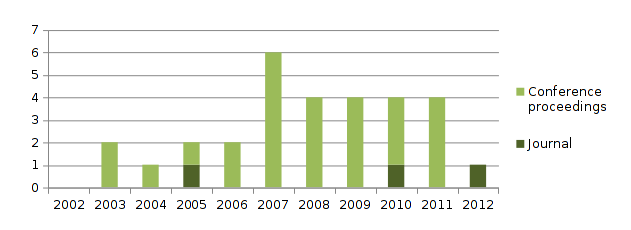
\includegraphics[width=1\textwidth]{img/Publications}
    \caption{Julkaistut tutkimukset vuosittain}
    \label{fig:publications}
  \end{center}
\end{figure}

Suurimmassa osassa ensisijaisia tutkimuksia oli ilmoitettu ajankohta, jolloin
muutoksen ensi askeleet oli otettu. Kuva~\ref{fig:start_year} esittää ilmoitetut
muutosten alkuajankohdat ryhmiteltynä vuosittain. Mediaani muutoksen
aloitusajankohdasta siitä kertoneen tutkimuksen julkaisuun oli kolme vuotta.
Tämä näkyy aloitettujen muutoshankkeiden nousussa vuonna 2004 ja julkaisujen
lukumäärän nousussa vuonna 2007. Tästä voidaan päätellä, että suuren mittakaavan
muutokset ketteriin menetelmiin ovat yleistyneet viime vuosikymmenen puolesta
välistä alkaen.

\begin{figure}[htb]
  \begin{center}
    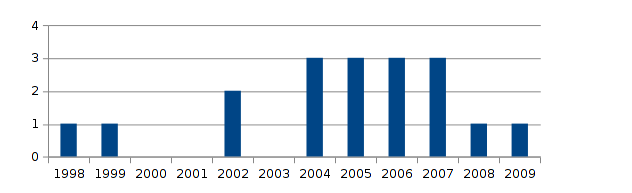
\includegraphics[width=1\textwidth]{img/Transformation_start}
    \caption{Organisaatiomuutosten aloitusajankohdat vuosittain}
    \label{fig:start_year}
  \end{center}
\end{figure}

\subsection{Käytetyt ketterät menetelmät}

Kaikissa tapauksissa organisaatio oli raportoidun ajanjakson lopussa edelleen
jatkanut ketterien menetelmien soveltamista. Muutoksen vaikutuksia oli
tyypillisesti raportoitu 1 tai 2 vuoden päähän sen aloittamisesta. Suurimmassa
osassa ensisijaisia tutkimuksia muutos katsottiin edelleen jatkuvan raportin
kirjoitusajankohtana.

Suurin osa ensisijaisista tutkimuksista erotteli käytössä olevia ketteriä
menetelmiä. Taulukko~\ref{table:practices} esittää suosituimmat menetelmät.
Ylivoimaisesti suosituin ketterä menetelmä oli Scrum, jota mainittiin
käytettävän miltei kahdessa kolmesta organisaatiosta. Toiseksi suosituin
menetelmä oli Extreme Programming. Osassa organisaatioista myös kevyt
kehitysmalli oli yhdistetty ketteriin menetelmiin.

Taulukosta~\ref{table:practices} ilmenee myös eri menetelmien yhdistely
huomattavana trendinä. Lähes kolmanneksessa ensisijaista tutkimuksista
mainittiin suoraan, että menetelmiä oli yhdistelty. Menetelmien yhdistelemistä
ja räätälöintiä oli perusteltu pääasiallisesti kahdella tapaa. Osalta syyksi oli
mainittu se, että suuren organisaation erityispiirteet tekivät menetelmän
räätälöinnin välttämättömäksi. Toisaalta yritykset olivat halunneet panostaa
mahdollisimman hyvän menetelmän löytämiseen, jolloin useita menetelmiä oli
arvioitu ja niiden sopivimmat piirteet oli yhdistetty.

\begin{table}[h]
    \begin{tabular}{ll}
        \toprule
        Menetelmä       & N   \\ \midrule
        Scrum           & 18 \\ 
        XP              & 7 \\
        Lean            & 5 \\
        Eri menetelmien yhdistely ja räätälöinti & 9  (epäsuorasti mainittuna useampia) \\
        \bottomrule
    \end{tabular}
	\caption{Hauissa käytetyt näkökulmat ja niitä vastaavat avainsanat. Sarake N
	kuvaa kuinka monessa tutkimuksessa menetelmää mainittiin käytettävän.}
	\label{table:practices}
\end{table}

Edellä mainittujen ketterien mallien lisäksi oli yksittäisiä mainintoja
seuraavista menetelmistä: JAD (Joint Application Development),
ASSF\footnote{Qumer ja Henderson-Sellers [S9] kuvaavat ASSF-menetelmän}, Unified
Process, sekä DSDM (Dynamic Systems Development Method). Näiden menetelmien
lisäksi mainittiin erilaisia käytäntöjä, mukaan lukien ajallinen rytmittäminen,
testivetoinen kehitys, asiakkaan mukanaolo, testauksen automatisointi, sekä
jatkuva yhdentäminen.

\subsection{Perusteet organisaatiomuutoksen aloittamiselle}

Ensisijaisissa tutkimuksissa raportoitiin kolmenlaisia perusteita muutokseen
ryhtymisellä. Suosituin perustelu oli yleinen tarve toiminnan tehostamiselle.
Tämän lisäksi perusteita olivat pyrkimys poistaa tiedostettuja ongelmia käytössä
olevasta prosessista, sekä tarve vastata nopeammin markkinoiden muutoksiin.
Kolmanneksessa tapauksista mainittiin, että organisaation johto oli havainnut
muutoksen tarpeen, ja tehnyt aloitteen muutokseen.

Seffernick [S10] kuvaa, että muutokseen päätettiin ryhtyä, sillä pakolla
määrätyt ja raskaat prosessit hidastivat tuotekehitystä, sekä heikensivät
asiakkaan tuotteesta saamaa arvoa. Petersen ja Wohlin [S27] kertovat, että
organisaation suorituskykyä verrattiin ohjelmistoteollisuuden parhaisiin
käytäntöihin, ja havaittiin, että tuotantoprosessi suoriutui heikosti. McDowell
ja Dourambeis [S7] kertovat, että organisaation toimiala oli murroksessa, ja
oli strategisesti välttämätöntä varustautua vastaamaan nopeisiin muutoksiin.
Qumer ja Henderson-Sellers [S9] kertovat, että muutokseen päätettiin ryhtyä kun
havaittiin että uusien toiminnallisuuksien kehittäminen käytössä olleella
menetelmällä oli hidasta ja heikensi yrityksen kilpailukykyä.

\subsection{Organisaatiomuutosten piirteet}

Ketterien menetelmien käyttöönottoon tähdänneitä organisaatiomuutoksia
tarkastellaan viidestä eri näkökulmasta, jotka ilmenivät ensisijaisista
tutkimuksista. Ensimmäiset näkökulmat ovat tapa jolla muutosta johdettiin ja
malli jolla muutosta toteutettiin. Muut keskeiset näkökulmat ovat
organisaatioiden tekemät sijoitukset organisaatiomuutokseen, miten
yhteisönrakentamisella pyrittiin ankkuroimaan muutosta sekä pilotoinnin käyttö.

\subsubsection{Muutoksen johtaminen}

Organisaation johdolla on keskeinen rooli muutoksissa, mikä näkyy siinä, että
suuressa osassa ensisijaisia tutkimuksia kerrotaan, että johto oli ensimmäisenä
käynnistänyt organisaatiomuutoksen. Useassa tapauksessa johto oli myös
vetovastuussa muutoksen läpiviemisestä. Esimerkiksi Goos ja Melisse [S4]
kertovat että johdon vahva osallistuminen oli tärkeää muutoksen juurruttamiseksi
ja oikean suunnan säilyttämiseksi, vaikka toimeenpaneva vastuu uusien
käytäntöjen luomisesta oli toteuttavalla portaalla. Myös Maples [S11] kuvaa,
miten tuotekehitys oli ottanut käyttöön ketteriä malleja tiimikohtaisesti, mutta
uusien käytäntöjen yhteensovittaminen ja koordinointi koko organisaation
laajuudessa vaati aloitetta johdon tasolla.

Organisaatiomuutos vaatii tahon jolla on vahvaa halua muutokseen, johtamiskykyä
ja vaikutusvaltaa. Useassa tapauksessa muutoksessa oli yksi keskeinen henkilö,
joka toimi muutoksen mestarina (engl. champion). Muun muassa O'Connor [S6]
esittää kuinka muutos aloitettiin uuden teknologiajohtajan toimesta, jolla oli
kokemusta aikaisemmista organisaatiomuutoksista. Myös Atlas [S1] raportoi
muutosta, jossa muutosta veti yksi asialle omistautunut henkilö. Kyseisessä
tapauksessa muutoksen mestari onnistui juurruttamaan muutoksen siten, että hän
pystyi lopuksi luovuttamaan muutoksen vetovastuun organisaatioon muodostuneelle
ketteriä menetelmiä edistävälle yhteisölle [S1]. Kahdessa tapauksessa
organisaatio palkkasi ulkopuolisen konsultin vetämään muutosta [S5, S30].

Joissakin tapauksissa organisaatiomuutosta ohjasi työryhmä johon oli koottu
useita eri näkökulmia edustavia jäseniä. Bang [S17] kertoo miten muutoksen
koordinointia varten perustettiin projektiryhmä, johon kuului jäseniä muun
muassa ylemmästä johdosta, myynnistä, projektijohdosta, ohjelmistokehityksestä
ja graafisesta suunnittelusta. Poikkiorganisatoorillisen työryhmän tärkeäksi
ominaisuudeksi raportoitiin se, että kaikkien osapuolten näkemyksiä kuullaan ja
vastakkainasetteluita sillataan [S15, S19].

\subsubsection{Muutoksen malli}

Yleisin malli josta ensisijaisissa tutkimuksissa raportoitiin oli ketterien
menetelmien askeleittainen käyttöönotto. Esimerkiksi Pertersen ja Wohlin [S27]
kertovat miten askeleittainen käyttöönotto toteutettiin ottamalla ensiksi
käyttöön pienet tiimit ja tuotteen kehitysjono (engl. product backlog), ja vasta
näiden ollessa toiminnassa siirryttiin soveltamaan muita käytäntöjä kuten
jatkuvaa prosessinparannusta ja päiväpalavereita (engl. stand-up meetings).
Wilby [21] kertoo että ketterä kehitys otettiin ensin käyttöön tiimitasolla,
jonka jälkeen todettiin että pitkän tähtäimen suunnittelu pitää myös muuttaa
ketteräksi. Myös Moore ja Spens [S23] esittävät miten suunnittelu muutettiin
joustavaksi ensin yksittäisten tiimien tasolla, mikä synnytti tarpeen kehittää
tehokkaampia tapoja hallita riippuvuuksiin vaikuttavia muutoksia ja tiimien
tuotosten yhdentämistä. Pilottiprojektit olivat myös suosittu tapa hallita
askeleittaista käyttöönottoa (katso kohta \ref{subsec:pilotointi}).

Vastakohtana askeleittaiselle käyttöönotolle eräässä organisaatiossa päädyttiin
muuttamaan kaikki kehitystiimit yhdellä kertaa käyttämään ketterää mallia.
Perusteluna yhdellä kertaa toteutetulle käyttöönotolle oli johdon pyrkimys
esittää vahvaa määrätietoisuutta muutoksessa, sekä toimintatapojen pitäminen
yhdenmukaisina. Kerralla toteutetun muutoksen raportoitiin onnistuneen. [S19]

Osassa organisaatioita muutoksen myötä päädyttiin malliin jossa yhdistettiin
aikaisempia toimintatapoja ja ketteryyttä. Esimerkiksi Karlström ja Runeson [S8]
kertovat miten ketterät menetelmät yhdistettiin Stage-Gate malliin, joka
helpotti tiimien välistä koordinointia sekä kommunikaatiota markkinoinnin ja
ylemmän johdon kanssa. Wilbyn [S21] kuvaamassa organisaatiossa alkuperäinen
vuosittainen roadmapping-käytäntö sovitettiin ketteräksi lyhentämällä
suunnitteluväliä neljännesvuoteen, ja ottamalla suunnitteluun mukaan edustajia
kaikilta organisaation osa-alueilta.

\subsubsection{Konsultointi, koulutus ja muut muutokseen liittyvät sijoitukset}
\label{sec:investments}

Ulkopuolisten konsulttien käyttö oli hyvin tyypillistä, ja siitä oli raportoitu
yli puolessa kaikista ensisijaisista tutkimuksista. Konsultteja käytettiin
erityisesti muutosprosessin suunnittelussa ja ketterän kehitysmallin
sovittamisessa organisaation tarpeisiin [S5, S10, S21, S23, S26, S29]. Konsultit
seurasivat usein organisaatiota läpi muutoksen ja toimivat tiimien valmentajina
(engl. coach) ketterää kehitystä varten [S4, S6, S19, S23, S30]. Konsultteja
käytettiin myös kouluttamaan organisaation sisäisiä ketterän kehityksen
valmentajia [S4, S28].

Koulutus oli keskeisessä osassa muutosta, ja suuri osa ensisijaisista
tutkimuksista raportoi siitä [S1, S5, S10, S16, S19, S22, S26, S30]. Jotkut
organisaatiot jopa räätälöivät oman opetussuunnitelman ketterien menetelmien
kouluttamiseen. Abernathy [S16] kertoo räätälöidyn opetussuunnitelman tuottaneen
niin hyviä tuloksia, että organisaatio päätti alkaa antaa koulutusta myös
ulkopuolisille tahoille. Koulutusta vahvistettiin useassa tapauksessa
erilaisilla työpajoilla, epävirallisilla tapaamisilla ja seminaareilla.
Esimerkiksi McDowell ja Dourambeis [S7] kuvaavat miten organisaatiossa
toteutettiin useita noin sadan osallistujan päivän mittaisia tapahtumia, jossa
harjoiteltiin ketterien menetelmien käyttöä. Tapahtumissa keskityttiin ketterien
menetelmien laajan käsittelyn sijaan vain tärkeimpien periaatteiden
opettamiseen, jotta osallistujat ymmärtäisivät ne hyvin [S7]. Seffernick [S10]
kertoo työpajoista, joilla vahvistettiin projektinjohdon ja tuoteomistajien
ymmärrystä ja innokkuutta ketterän mallin käyttöön.

Muutos ketterään malliin merkitsi toimintatapojen muuttamisen lisäksi myös
fyysisten tilojen uudelleenjärjestämistä. Seffernick [S10] raportoi että
työpisteet uudelleenjärjestettiin muodostamaan tiimihuoneita, ja lisäksi
rakennettiin pelihuone ja kahvila yleisiin tiloihin. Heidenberg et al. [S26]
kertoo työtilan järjestelyn tiimihuoneiksi vieneen enemmän tilaa henkilöä kohden
kuin tavanomaisessa toimistotilassa, mikä vaati lisäresursointia.

Ketterä kehitys vaati myös panostusta uusiin työkaluihin. Esimerkiksi Fry ja
Greene [S19] sekä Ryan ja Scudiere [S29] raportoivat wiki-järjestelmän
käyttöönotosta tiedonjakamisen helpottamiseksi. Ensisijaisissa tutkimuksissa
kerrottiin myös panostuksista laadunvarmistuksen työkaluihin. Fry ja Greene
[S19] kertovat myös miten testausautomaation rakentaminen oli keskeisenä
tekijänä ketterien menetelmien soveltamisessa. Moore ja Spens [S23] raportoivat
merkittävästä panostuksesta testaukseen sekä jatkuvan yhdentämisen työkaluihin.

\subsubsection{Yhteisöllisyyden rakentaminen}

Yhteisöllisyyden rakentamista käsiteltiin tärkeänä asiana suuressa osassa
ensisijaisia tutkimuksia. Yhteisöllisyyden luominen uusien työtapojen ympärille
on keskeistä muutoksen juurruttamisen kannalta. Esimerkiksi Abernathy [S16]
kuvaa miten organisaatiossa pyrittiin luomaan yhteisöjä eri osaamisen, muun
muassa testauksen, arkkitehtuurin ja järjestelmäanalyysin, alueilla.
Näiden yhteisöjen tarkoitus oli levittää tietoa, osaamista ja uusia työtapoja
yli organisaation sisäisten rajojen [S16]. Atlas [S1] kertoo miten muutoksen
mestari onnistui muodostamaan yhteisön uuden toimintamallin ympärille siten,
että hän itse pystyi väistymään johtavasta roolista ketterien menetelmien
edistämisessä.

Valmentamista voidaan pitää eräänä yhteisöllisyyden muotona. Valmentaja toimii
uuden menetelmän puolestapuhujana, ja avustaa tiimejä menetelmän käytännön
soveltamisessa. Muun muassa Silva ja Doss [S28] kuvaavat miten valmentaminen oli
tärkeä toiminto ketterien menetelmien käyttöönotossa, ja miten myös valmentajat
muodostivat oman yhteisönsä. Myös Benefield [S22] mainitsee valmennuksen
tärkeyden.

\subsubsection{Pilottihankkeiden soveltaminen}
\label{subsec:pilotointi}

Pilotoinnin soveltaminen oli tyypillistä muutoksen alussa. Pilottiprojektien
keskeinen vaikutus oli myönteisen asenteen muodostuminen ketterää kehitystä
kohtaan [S4, S6, S8, S10, S24, S26, S28]. Toinen pilottiprojektien tavoite oli
uuden prosessin ja työkalujen räätälöinti ja arviointi [S4, S14, S26].
Useassa organisaatioissa suoritettiin monta pilottiprojektia [S4, S22, S24,
S28]. Syynä oli muun muassa se, että projektien katsottiin eroavan toisistaan,
ja tarvittiin todisteita ketterien menetelmien laaja-alaisesta
sovellettavuudesta [S26]. Eräässä organisaatiossa päädyttiin suorittamaan
pilottiprojektit liiketoiminnan kannalta kriittisissä projekteissa, joihin ei
saanut aiheutua keskeytyksiä [S4].

Pilotoinnin suunnitteluun liittyi myös haasteita. O'Connor [S6] kertoo miten
erittäin suotuisan ympäristön luominen pilottiprojektille ja erinomaiset
lopputulokset loivat epärealistisia odotuksia. Tämä johti käyttöönoton
laajentuessa turhautumiseen, kun samoja tuloksia ei enää kyetty saavuttamaan.

\subsection{Ongelmia ketterän kehityksen käyttöönotossa}

Onnistuneen ketterien käyttöönotossa esiintyneitä haasteita listataan neljässä
eri kategoriassa. Ensimmäiseksi käsitellään ongelmia saavuttaa hyväksyntä ja
yhtenäinen suunta muutokselle. Toisena kategoriana esitellään ketterien
menetelmien väärinymmärryksestä johtuneita ongelmia. Kolmas kategoria on
ketterän mallin soveltumattomuus ja ristiriidat organisaation eri ryhmien
välillä. Neljänneksi käsitellään haasteita jotka ovat aiheutuneet
puutteellisesta resursoinnista ja varautumisesta muutokseen.

\subsubsection{Organisaation yhtenäinen suuntaaminen muutoksessa}

Muutoksen johtamisen kannalta haasteeksi nousi usein yhtenäisen suunnan
saavuttaminen muutoksessa. Yhtenäisyyden puutteen oireiksi voidaan tulkita
johdon tuen puuttuminen, muutosvastarinta ja liika innokkuus. Hajjdiab et al.
[S5] kertovat miten johdon tuen puuttuminen vähensi henkilöstön motivaatiota
panostaa muutokseen ja hankaloitti muutokseen vaatimaa resursointia. Spayd [S13]
kuvaa, että vaikka kehittäjille oli järjestetty koulutusta, keskijohdolle ei
ollut suunniteltu sopivaa koulutusohjelmaa, jonka seurauksena ymmärryksen
puute muodostui suurimmaksi muutosta haittaavaksi tekijäksi.

Muutosvastarintaa syntyi muun muassa tiimitilojen uudelleenjärjestelystä [S14].
Hallikainen [S14] kertoo että muutosvastarintaa poistettiin suurella
panostuksella henkilökohtaisiin keskusteluihin johtajien ja henkilöstön välillä.
Heidenberg et al. [S26] kertoo että muutosvastarintaa pyrittiin lieventämään
pilotoinnilla. Benefield [S22] esittää että tilanteesta riippumatta on
hyväksyttävä ja varauduttava siihen, että 10-15 \% henkilöstöstä ei ole
tyytyväisiä käytössä oleviin toimintatapoihin.

Muutosvastarinnan vastakohtana yli-innokkuus aiheutti myös ongelmia. Muun muassa
Hajjdiab et al. [S5] sekä O'Connor [S6] kuvaa miten yli-innokkuus johti 
kiinnostuksen menettämiseen ja turhautumiseen. Benefield [S22] kuvaa miten
ketterien menetelmien valmentajia piti ohjata välttämään menetelmien
määräämistä, ja sen sijaan antamaan suosituksia, jotta heitä ei tulkittaisi
yli-innokkaiksi ja epäuskottaviksi.

Useassa tapauksessa ketterää muutosta uhkasi vanhan toimintamallin palaaminen.
Muun muassa Goos ja Melisse [S4] kertoivat kehittäjien palaavan
aikataulupaineen alla käyttämään vanhasta mallista tuttuja käytäntöjä. Myös
arkkitehtuurilliset yhdentämisvaikeudet eri osastojen välillä johtivat
sopimuspohjaisen menettelyn paluuseen [S23]. Maples [S11] kuvasi että tuotteen
julkaisuprosessia ei oltu muutettu ketteräksi, ja se vaati julkaistavien
ominaisuuksien lukitsemisen 90 päivää etukäteen. Ominaisuuksien lukitseminen
aiheutti määräilevän johtamistyylin paluuta, mikä soti ketteriä periaatteita
vastaan [S11].

\subsubsection{Uuden mallin väärinymmärtäminen}

Ketterien menetelmien soveltaminen väärin oli yleinen ongelma. Esimerkiksi
Benefield kuvaa miten jotkut tiimit väittivät käyttävänsä ketteriä menetelmiä,
mutta tekivät todellisuudessa pienoiskokoista vesiputouskehitystä. Syyksi tähän
Benefield mainitsee puutteellisen koulutuksen resurssipulan takia.
Projektipäälliköt käyttivät myös Scrum-termistöä, mutta todellisuudessa jakoivat
työtehtäviä määräilevästi, ja tekivät sitoumuksia kuulematta tiimiä. [S22]

Myös Seffernick [S10] kuvaa miten vanhan mallin rooleja sovitettiin
Scrum-malliin muuttamatta kuitenkaan todellisia toimintatapoja, mikä ei
edistänyt toimintamallin muutosta. Maples [S11] kertoo miten kaikkien osapuolten
kuuleminen ymmärrettiin väärin siten, että tuotteen kehitysjonoon tulvi liikaa
vaatimuksia, mikä johti vaatimusten kauppaamiseen ja epätehokkaaseen
priorisointiin. Abernathy [S16] kuvaa miten linjapäälliköt ohittivat
tiimikohtaisen projektipäällikön, ja puuttuivat tiimien sisäisiin asioihin,
mikä johti luottamuspulaan ja haittasi ketterän mallin toteuttamista.

\subsubsection{Soveltuvuus ja ristiriidat organisaation muiden ryhmien kanssa}

Monessa tapauksessa ketterä kehitys saatiin toimimaan yksittäisten tiimien
tasolla, mutta ongelmia alkoi esiintyä kun ketterää mallia alettiin soveltaa
laajemmin. Maples [S11] kertoo, että markkinointiosasto joutui törmäyskurssille
tuotekehityksen kanssa kun ketterien menetelmien käyttöä laajennettiin, sillä
vanhassa kehitysmallissa markkinointi vaati suunnitelmien lukkoon lyömistä
pitkällä tähtäimellä. Myös vientilupien ja kolmannen osapuolen lisenssien
hankkiminen vaati suunnittelua pidemmällä aikavälillä. Lopputuloksena
muodostettiin malli jossa markkinoinnin sallitaan määrittää julkaisupäivä tietty
aika etukäteen, ja tuotekehitys sitoutuu toimittamaan tietyt toiminnallisuudet
siihen mennessä [S11]. Myös O'Connor [S6] kertoo kuinka organisaation johto
vaati pidemmän tähtäimen suunnitelmia, joita oli ongelmallisia toimittaa
ketterän kehityksen puitteissa. Eräässä tapauksessa johto ja myyntiosasto
tukivat ketterää kehitystä pyrkimällä päivittämällä sopimuskäytäntöjä sallimaan
ketteryyttä paremmin [S17]. Moore ja Spens [S23] kertovat kuinka ketterässä
kehityksessä käytetty joustavampi suunnittelu salli muutoksia, jotka aiheuttivat
laatuongelmia kun projektien tuotoksia yhdennettiin.

Joissakin organisaatioissa havaittiin, että ketterä kehitys ei sovellu
laajennettavaksi kaikkiin toimintoihin. Muun muassa Korhonen [S2] kertoo että
Scrum-käytännöt eivät soveltuneet testaukseen ja tukitoimintoihin. Tukitiimin
toimintatapa vaati välitöntä vastaamista ongelmiin, eikä ajallisen rytmittämisen
periaatteita voitu soveltaa [S2]. Myös Spayd [S13] esitti ketterien mallien
havaittiin soveltuvan huonosti ylläpitokehitykseen. Ylläpitotiimit samaistuivat
kuitenkin käynnissä olevaan muutokseen, ja menetelmien tarkempi räätälöinti
jätettiin tulevaisuuteen [S13]. Goos ja Melisse [S4] havaitsivat että ketterät
menetelmät soveltuivat organisaation toimintoihin sitä huonommin mitä kauempana
tuotekehityksestä ne oli.

Benefield [S22] raportoi että organisaation hallinto-osastot kuten
henkilöstöhallinto ja matriisiorganisaation johto asettivat toimintatavoillaan
haasteita ketterälle kehitykselle. Edellä mainitut osastot pyrkivät
hallinnoimaan työntekijöitä yksilötasolla, mikä haittasi ketterien menetelmien
tiimikeskeistä toimintatapaa [S22]. Spayd [S13] kertoo kuinka henkilöstöhallinto
esti tiimikohtaisen palkitsemisen, sekä tilahallinto esti tiimejä muodostamasta
yhteisiä tiloja.

\subsubsection{Puutteellinen varautuminen muutokseen}

Suurimmaksi resursointiongelmaksi muodostui valmennuksen ja koulutuksen puute.
Esimerkiksi Benefield [S22] raportoi että osaavien valmentajien puute hidasti
ketterien menetelmien käyttöönoton laajentamista. Silva ja Doss [S28]
käsittelevät haasteita uusien valmentajien koulutuksessa, kun valmennuksen tarve
kasvoi voimakkaasti uuden kehitysmallin yleistyessä. Valmentajakoulutukseen
hakeutuneet henkilöt olivat usein tottuneita perinteiseen ohjelmistokehityksen
malliin, mikä aiheutti riskin, että uudet valmentajat olisivat levittäneet
väärin käsitettyä ketterän kehityksen mallia [S28]. Myös Spayd [S13] raportoi
puutteellisesta koulutuksesta, jonka takia ketteriä periaatteita ei ymmärretty
ja sovellettiin epätehokkaasti.

\subsection{Muutosprosessin menestyksen tekijät}

Ensisijaisista tutkimuksista tunnistettiin neljä tekijää jotka edesauttoivat
muutosprosessin menestystä. Ensimmäinen tekijä on organisaation yhdenmukainen
suuntaaminen ja muutoksen johtaminen. Muutoksen suunnitteleminen on toinen
tekijä joka esitellään. Kolmanneksi esitellään hyviä käytäntöjä uuden
toimintatavan soveltamisessa. Neljäntenä tekijänä on riittävä resursointi
muutoksen läpiviemiseen.

\subsubsection{Organisaation yhdensuuntaistaminen ja muutoksen johtaminen}

Johdon vahva tuki on tärkeä tekijä menestyneessä organisaatiomuutoksessa.
Muun muassa Abernathy [S16] painottaa ylimmän johdon roolia muutoksessa. Myös
johdon on ymmärrettävä ketterän kehityksen perusteet, jonka takia johdon on
osallistuttava koulutukseen [S16]. Spayd [S13] ehdottaa että johdon kannattaa
pyrkiä niin kutsuttu luomaan palavan lautan (engl. burning platform) vaikutus,
jossa annetaan vahva ymmärrys siitä, että vanhaan toimintamalli on tuhoon
tuomittu.

Johdon tulee kuitenkin välttää määräävää tai muutokseen pakottavaa asennetta.
Atlas [S1] kertoo, että henkilöstö kiinnostui itsestään Scrum-menetelmän
käytöstä kun heille annettiin tietoa siitä. Benefield [S22] kuvaa miten
yritykset saada tiimit käyttämään ketterää menetelmään määräyksen kautta
epäonnistuivat aina.

Muutossuunnitelmien ja vision kommunikointi on tärkeä osa vahvistaa muutoksen
kannatusta henkilöstön keskuudessa. Fry ja Greene [S19] kertovat tiedotuksen ja
läpinäkyvyyden olleen avaintekijä muutoksen onnistumisessa. Muutoksen visiota ja
tilaa ylikommunikoitiin jatkuvasti, muun muassa esittämällä kaikki
muutossuunnitelmat ja pitämällä muutoksen ohjaamiseen liittyvät kokoukset
yleisissä tiloissa [S19]. McDowell ja Dourambeis [S7] kuvaavat miten
organisaatiossa panostettiin suuren mittakaavan tilaisuuksiin, joissa
tiedotetaan muutoksesta. Muita tapoja nostaa kannatusta muutokseen on osallistaa
henkilöstöä muutoksen tekemiseen. Hallikainen [S14] kertoo miten tiimien
annettiin itse päättää muun muassa uusien työtilojen suunnittelusta.

Hyvien tulosten saavuttamiseksi on tärkeää tuoda yhteen organisaation eri
ryhmät. Baker [S15] kertoo miten muutoksen suunnitteluun muodostettiin työryhmä
jossa oli osallistujia jokaisesta organisaation osasta jota muutos koski.
Työryhmän tavoite oli mukanaolon lisäksi synnyttää vahvaa yhteistyötä
organisaation eri osien välillä [S15]. Myös Wilby [S21] kuvaa miten
organisaation sisäinen yhteistyötä saatiin parannettua merkittävästi kun pitkän
tähtäimen suunnitteluun kehitettiin kaikkia organisaation osapuolia kuuleva
työryhmämenettely.

\subsubsection{Panostaminen valmennukseen ja yhteisöllisyyteen}

Valmennus on välttämätöntä ketterien menetelmien soveltamisessa, sillä tiimeillä
ei ole lähtökohtaisesti vahvaa osaamista ketterien menetelmien soveltamisessa.
Ketterät menetelmät perustuvat itseohjautuvuuteen, jonka takia määräävää
ohjaaminen on korvattava valmennuksella. Esimerkiksi Atlas [S1] kertoo että
tiimit joilla oli ongelmia ketterän kehityksen kanssa eivät olleet saaneet
valmennusta, kun taas valmennusta saaneet tiimien tarvitsi harvoin pyytää apua.
Silva ja Doss [S28] suosittelevat että johtoa muistutetaan jatkuvasti
valmennuksen tärkeydestä, jotta pätevän valmentajien yhteisön ylläpitämiseen
panostetaan.

Uuden menetelmän juurruttaminen isoon organisaatioon on haastavaa, mutta
muutoksen pysyvyyttä voi parantaa luomalla yhteisöjä uuden menetelmän ympärille.
Jatkuva menetelmän parantaminen on keskeistä ketterässä kehityksessä, ja on
tärkeätä muodstaa yhteisöjä joissa kehitysehdotuksista keskustellaan.
O'Connor [S6] kertoo miten jatkuvaa kehittymisen ilmapiiriä vahvistetaan
yhteisöllisyydellä ja tiedon jakamisella. Organisaatiossa järjestetään muun
muassa lounasseminaareja ja koko päivän mittaisia tapahtumia joissa kehitetään
henkilöstön taitoja [S6]. Kähkönen [S3] esittää että yhteisöllisyys helpottaa
ketterien menetelmien käyttöönottoa suurissa orgainsaatioissa. Yhteisöjen
luomista voi helpottaa muun muassa järjestämällä ohjattuja tiimienvälisiä
työpajoja [S3].

\subsubsection{Menetelmien sovittaminen ja yhdenmukaisuus}

Kirjallisuudessa esiteltyjä menetelmiä kannattaa aina soveltaa organisaation
tarpeisiin. Erityisesti suuressa mittakaavassa on tarve sovittaa ketteriä
menetelmiä, sillä niissä otetaan harvoin huomioon suurten organisaatioiden
erityistarpeita. Muun muassa Maples [S11] kuvaa miten tuotteen kehitysjonon
käsittelyä sekä korkean tason testausta oli tarve sovittaa. Tärkeä sovittamista
vaativa osa-alue oli johtajien roolien mukauttaminen ketterään kehitykseen.
Yi [S20] kuvaa miten linjapäällikön rooli yhdistettiin Scrum-mestarin rooliin.
Tämä saattaa vaikuttaa ristiriitaiselta, sillä Scrum-mestarin tehtävä on
pikemmin tiimin avustaminen kuin päällikkönä toimiminen, mutta Yi perustelee
valintaa sillä, että tiimeistä ei voi tulla itseohjautuvia toimi ellei myös
johto muuta rooliaan ketteräksi [S20]. 

Useassa tapauksessa raportoitiin yhdenmukaisten toimintatapojen eduista.
Muun muassa Fry ja Greene [S19] tuo esille yhdenmukaisen sanaston käyttämisen
etuna. Benefield [S24] kertoo että työkalujen ja käytäntöjen standardointi
helpotti tiedon jakamista tiimien kesken ja yhteisöllisyyden vahvistamista. Ryan
ja Scudiere [S29] kertovat että uusien menetelmien soveltaminen ilman
pelisääntöjä johti aina epäonnistumiseen. Tämän perusteella tiimeille asetettiin
muutamia yhteisiä pakollisia ketteriä käytäntöjä, mikä osoittautui erittäin
tehokkaaksi tavaksi yhtenäistää organisaatiota muutoksessa [S29]. Tudor ja
Walter [S30] esittävät etuna sen, että selkeästi määritelty prosessi loi
yhteisen käsitteistön, ja antoi syyn pysyä DSDM-menetelmässä, vaikka uusia
ketteriä menetelmiä esiteltiin ajan myötä.

Muutamat ensisijaiset tutkimukset kuvasivat miten kiintopisteiden asettaminen
edistää organisaatiomuutosta. Spayd [S13] kertoo että uuden version julkaisu 90
päivän välein loi tiukat kiintopisteet, ja antoi muutokselle selkeän rytmin.
Myös Ryan ja Scudiere [S29] kuvaavat että tiukkojen julkaisupäivien asettaminen
antoi liiketoiminnalle uskoa pitkien suunnitelmien puuttuessa, ja suuntasi koko
organisaation yhteistä selkeää tavoitetta kohden.

\subsubsection{Muutokseen vaatimat sijoitukset}

On selvää että laajan organisaatiomuutoksen läpivieminen vaatii enemmän
panostuksia kuin organisaation normaali toiminta. Osa-alueita joihin
panostaminen oli raportoitu erityisen tärkeäksi oli koulutus ja ulkopuolisten
konsulttien käyttö. Näiden lisäksi oli menestyksen tekijöinä raportoitu
panostuksia testauksen automatisointiin, jatkuvaan yhdentämiseen sekä
toimistotilojen muokkaamiseen. Edellä mainittujen tekijöiden soveltamista
on kuvattu luvussa \ref{sec:investments}.


% --------------------------------------------------------------------
\clearpage
\section{Yhteenveto}
\label{sec:johtopaatokset}

Tämän työn tavoitteena oli selvittää mitkä tekijät vaikuttavat ketterän
kehitysmallin organisaatiomuutoksen läpiviemiseen suuressa organisaatiossa,
miten muutokset yleensä toteutetaan sekä miksi muutokseen ryhdytään. Hyödyntäen
järjestelmällisen kirjallisuustutkimuksen menetelmää löydettiin 30 ensisijaista
tutkimusta, jotka antoivat vastauksia tutkimuskysymyksiin. Esitellyissä
tuloksissa tehtiin ensin yhteenveto lähdemateriaalista, jonka jälkeen esiteltiin
tyypillisiä muutoksen toteutustapoja, haasteita ja menestyksen tekijöitä.

Organisaatiomuutokseen ryhdyttiin kolmesta pääasiallisesta syystä, joita olivat
yleinen tarve tehostaa toimintaa, tiedostettujen prosessiongelmien poistaminen
ja tarve vastata markkinoiden muutoksiin nopeammin. Organisaatiomuutoksen
keskeisimmäksi tekijäksi nousi tapa, jolla muutosta johdettiin. Määrätietoinen
johtaminen oli keskeisin menestyksen tekijä muutoksessa. Keskeisimmät ongelmat
johtuivat vaikeuksista muodostaa yhtenäistä suuntaa muutokselle kautta
organisaation. Muita tärkeitä menestyksen tekijöitä oli riittävä koulutuksen
järjestäminen sekä yhteisöllisyyden luominen. Pilotointi ja ulkopuolisten
konsulttien käyttö oli tyypillistä muutoksissa.

Tulosten perusteella ei voida antaa suoraviivaista suositusta miten muutos
kannattaisi toteuttaa, sillä kullakin organisaatiolla on erityispiirteitä jotka
vaikuttavat muutokseen. Yllä listatut haasteet ja menestyksen tekijät korostavat
kuitenkin muutamia muutokseen liittyviä osa-alueita, joihin kannattaa kiinnittää
huomiota kaikissa organisaatioissa.

Työn tuloksiin pitää suhtautua varauksella ja olettaa vääristymää esitetyissä
tuloksissa. Vääristymää on saattanut aiheuttaa se, että suurimmassa osassa
ensisijaisia tutkimuksia julkaisija kuului organisaatioon jonka muutosta
kuvattiin. Sen lisäksi suurin osa materiaalista oli kokemusraportteja ja
harvassa ensisijaisessa tutkimuksessa oli sovellettu tutkimusmenetelmää. Näiden
tekijöiden voidaan olettaa johtavan ongelmien vähättelyyn ja positiivisten
tulosten ylikorostamiseen, jonka takia tuloksia ei pidä tulkita
yksityiskohtaisesti. Tämä työ antaa kuitenkin arvokkaan yleiskatsauksen
raportoidusta muutoksista, sekä kartoittaa muutoksen osa-alueita joista
keskustellaan yleisimmin.

Suurten organisaatioiden erityispiirteitä ei verrattu pienten organisaatioiden
ketterän kehityksen malliin. Voidaan kuitenkin olettaa että tässä työssä
esitetyt tulokset liittyvät erityisesti suuriin organisaatioihin. Muutoksen
johtaminen suuressa mittakaavassa, yhteisöllisyyden rakentaminen sekä
ristiriidat tuotekehityksen ja organisaation muiden ryhmien välillä ovat tässä
työssä esille tulevia näkökulmia, jotka koskevat erityisesti kehitysmenetelmien
soveltamista suurissa organisaatioissa. Osa muutoksen tekijöistä voidaan olettaa
kuuluvan sekä pieniin että suuriin muutoshankkeisiin, mukaan lukien koulutuksen
ja konsultoinnin käyttö, pilottihankkeet, sekä uuden mallin väärinymmärtäminen.

Suositeltava jatkotutkimus on laajentaa tätä työtä seuraten huolellisesti
jotakin kirjallisuustutkimuksen menetelmää. Tämän työn sisältämä tutkimus on
sovitettu kandidaatintyön laajuuteen, jonka takia jouduttiin karsimaan useita
oleellisia menetelmään kuuluvia muodollisuuksia, kuten hakujen riippumaton
katselmointi. Toinen rajoitus tässä työssä oli muutoksen tarkasteleminen
pelkästään ohjelmistokehityksen näkökulmasta. Yleinen muutoksen johtaminen ja
suuret organisaatiomuutokset ovat laajalti tutkittuja aloja. Kiinnostava
jatkotutkimuksen osa-alue olisi vertailla ketterien menetelmien käyttöönottoa
yleisiin organisaatiomuutosten ja muutoksen johtamisen tutkimuksiin.


\clearpage
\large
\textbf{Menestyksekkään käyttöönoton tekijöitä (tausta)}
\normalsize

--> Muutoksen ydinalueiden tunnistaminen ja niihin keskittyminen (Misra)

\citeppri{Boehm2005}: --> -->
--> Ihmislähtöisyys on ketterien menetelmien lähtökohta. Ihmisten välinen
interaktio on avaintekijä ketterässä kehityksessä. Tämä on huomioitava
johtamisen tyylissä, joka on perinteisissä organisaatioissa usein määräävä. On
myös oletettavaa, että osa henkilöstöstä ei halua muuttaa toimintatapojaan.
Näiden haasteiden selvittäminen vaatii henkilöstön kouluttamista, sekä
ymmärrystä siitä, miten ihmisten väliset interaktiot luovat sujuvaa
kommunikaatiota. ? ? ?

\vspace{1cm}
\large
\textbf{Menestyksekkään käyttöönoton tekijöitä (tulokset)}
\normalsize

\textbf{Sovitus}

Menetelmien sovittaminen organisaation erityispiirteisiin on tärkeää, sillä -->
Goos ja Melisse [S4]: vaikka johto teki päätöksen muutokseen ryhtymisestä
muutoksen toteuttamisen lähtökohdat oli tiimitasolla. ???

\textbf{Resursointi}

--> Ulkopuolisten resurssien hyödyntäminen. (2 viitettä)

Koulutus oli tärkeä menestyksen tekijä monessa raportoidussa muutosprosessissa.
Muun muassa Karlström ja Runeson [S8] kertovat että koulutus oli tärkeä tekijä
muutosvastarinnan poistamisessa.

Spayd [S13] esittää että koulutus on tärkeää --> empowerment

\vspace{1cm}
\large
\textbf{Muita ideoita tuloksista}
\normalsize

\textbf{Muutoksen malli}

\hl{--> Oleellinen muutoksen vaikuttava} tekijä oli organisaation muut toiminnot
joiden kanssa ketterät ohjelmistokehitystiimit joutuvat kommunikoimaan.
--> (13 viitettä ja esimerkkiä)

\textbf{Muuta muutoksen piirteistä}

\hl{--> Lopputuloksena oli ketterien menetelmien} pysyvä käyttöönotto, paitsi [S5]
jossa organisaatio alkoi palata käyttämään vanhaa menetelmää. Yhdessä
tapauksessa ketterien menetelmien pilottiprojekti keskeytettiin
organisaation yleisen taloustilanteen takia [S26].
